% Options for packages loaded elsewhere
\PassOptionsToPackage{unicode}{hyperref}
\PassOptionsToPackage{hyphens}{url}
\PassOptionsToPackage{dvipsnames,svgnames,x11names}{xcolor}
%
\documentclass[
  12pt,
]{article}
\usepackage{amsmath,amssymb}
\usepackage{lmodern}
\usepackage{iftex}
\ifPDFTeX
  \usepackage[T1]{fontenc}
  \usepackage[utf8]{inputenc}
  \usepackage{textcomp} % provide euro and other symbols
\else % if luatex or xetex
  \usepackage{unicode-math}
  \defaultfontfeatures{Scale=MatchLowercase}
  \defaultfontfeatures[\rmfamily]{Ligatures=TeX,Scale=1}
\fi
% Use upquote if available, for straight quotes in verbatim environments
\IfFileExists{upquote.sty}{\usepackage{upquote}}{}
\IfFileExists{microtype.sty}{% use microtype if available
  \usepackage[]{microtype}
  \UseMicrotypeSet[protrusion]{basicmath} % disable protrusion for tt fonts
}{}
\makeatletter
\@ifundefined{KOMAClassName}{% if non-KOMA class
  \IfFileExists{parskip.sty}{%
    \usepackage{parskip}
  }{% else
    \setlength{\parindent}{0pt}
    \setlength{\parskip}{6pt plus 2pt minus 1pt}}
}{% if KOMA class
  \KOMAoptions{parskip=half}}
\makeatother
\usepackage{xcolor}
\usepackage[left=3cm,right=2cm,top=2cm,bottom=2cm]{geometry}
\usepackage{graphicx}
\makeatletter
\def\maxwidth{\ifdim\Gin@nat@width>\linewidth\linewidth\else\Gin@nat@width\fi}
\def\maxheight{\ifdim\Gin@nat@height>\textheight\textheight\else\Gin@nat@height\fi}
\makeatother
% Scale images if necessary, so that they will not overflow the page
% margins by default, and it is still possible to overwrite the defaults
% using explicit options in \includegraphics[width, height, ...]{}
\setkeys{Gin}{width=\maxwidth,height=\maxheight,keepaspectratio}
% Set default figure placement to htbp
\makeatletter
\def\fps@figure{htbp}
\makeatother
\setlength{\emergencystretch}{3em} % prevent overfull lines
\providecommand{\tightlist}{%
  \setlength{\itemsep}{0pt}\setlength{\parskip}{0pt}}
\setcounter{secnumdepth}{5}
\usepackage{mathtools}
\usepackage{amsmath}
\numberwithin{equation}{section}
\numberwithin{table}{section}
\numberwithin{figure}{section}
\usepackage{float}
\usepackage{gensymb}
\usepackage{setspace}\singlespacing
\usepackage{titlesec}
\titlespacing*{\section}{0pt}{3cm}{1cm}
\usepackage[nottoc]{tocbibind}
\setcounter{secnumdepth}{2}
\setcounter{tocdepth}{2}
\widowpenalties 3 10000 10000 150
\displaywidowpenalties 3 10000 10000 150
\clubpenalties 3 10000 10000 150
\interfootnotelinepenalty 5000
\raggedbottom
\usepackage{enumitem}
\setlist{itemsep=3pt,topsep=5pt,parsep=0pt,partopsep=0pt}
\usepackage{hyperref}
\hypersetup{bookmarksnumbered=true}
\usepackage{bookmark}
\newcommand{\sectionbreak}{\clearpage\phantomsection}
\let\Begin\begin
\let\End\end
\newcommand{\Newrow}{\\}
\AtBeginDocument{\pdfbookmark[section]{Deckblatt}{front}}
\usepackage{booktabs}
\usepackage{longtable}
\usepackage{array}
\usepackage{multirow}
\usepackage{wrapfig}
\usepackage{float}
\usepackage{colortbl}
\usepackage{pdflscape}
\usepackage{tabu}
\usepackage{threeparttable}
\usepackage{threeparttablex}
\usepackage[normalem]{ulem}
\usepackage{makecell}
\usepackage{xcolor}
\ifLuaTeX
  \usepackage{selnolig}  % disable illegal ligatures
\fi
\usepackage[]{natbib}
\bibliographystyle{agsm}
\IfFileExists{bookmark.sty}{\usepackage{bookmark}}{\usepackage{hyperref}}
\IfFileExists{xurl.sty}{\usepackage{xurl}}{} % add URL line breaks if available
\urlstyle{same} % disable monospaced font for URLs
\hypersetup{
  pdftitle={Asessing China's Climate Responsibility},
  pdfauthor={Johann-Friedrich Salzmann},
  colorlinks=true,
  linkcolor={MidnightBlue},
  filecolor={Maroon},
  citecolor={MidnightBlue},
  urlcolor={MidnightBlue},
  pdfcreator={LaTeX via pandoc}}

\title{Asessing China's Climate Responsibility\\
\strut \\
\strut \\
\strut \\}
\usepackage{etoolbox}
\makeatletter
\providecommand{\subtitle}[1]{% add subtitle to \maketitle
  \apptocmd{\@title}{\par {\large #1 \par}}{}{}
}
\makeatother
\subtitle{\textbf{Final Paper}\\
\strut \\
\strut \\
GRAD-E1402\\
Data Perspectives on GHG Emissions\\
Hertie School of Governance\\
\strut \\}
\author{submitted by\\
Meier, Constantin\\
Metz, Fabian\\
Mohn, Anna\\
Salzmann, Johann-Friedrich\\
\strut \\}
\date{12 December 2022}

\begin{document}
\maketitle

\renewcommand{\harvardand}{\&}
\setcitestyle{authoryear,round,aysep={},notesep={: }}

\thispagestyle{empty}
\pagenumbering{gobble}

\newpage
\pdfbookmark[section]{List of Abbreviations}{decl}
\section*{List of Abbreviations}
\thispagestyle{empty}
\pagenumbering{arabic} 
\onehalfspacing

\begin{table}[!ht]
    \centering
    \begin{tabular}{|l|l|}
    \hline
        AFOLU &  Agriculture, Forestry, Land Use  \\ \hline
        CAT &  Climate Action Tracker  \\ \hline
        CBRD &  Common but differentiated responsibilities and respective capabilities  \\ \hline
        COP &  Conference of the Parties  \\ \hline
        EDGAR &  Emissions Database for Global Atmospheric Research  \\ \hline
        GDP &  Gross domestic product  \\ \hline
        GHG &  Greenhouse gas  \\ \hline
        GNI &  Gross national income  \\ \hline
        GW &  Gigawatt  \\ \hline
        NDC &  Nationally determined contributions  \\ \hline
        REDD+ &  Reducing Emissions from Deforestation and Forest Degradation  \\ \hline
        UNFCCC & United Nations Framework Convention on Climate Change \\ \hline
    \end{tabular}
\end{table}

\singlespacing
\newpage
\pdfbookmark[section]{\contentsname}{toc}
\tableofcontents
\thispagestyle{empty}
\onehalfspacing

\hypertarget{introduction}{%
\section{Introduction}\label{introduction}}

\nocite{R-rmarkdown,R-tidyverse,R-eurostat,R-WDI,R-plotly,R-imputeTS,R-kableExtra}
\citet{WorldBank2022a} \citet{WorldBank2022b} \citet{Worldbank2022c}
\citet{Giacomo2022}

\hypertarget{data-assumptions}{%
\section{Data \& Assumptions}\label{data-assumptions}}

\hypertarget{used-data}{%
\subsection{Used Data}\label{used-data}}

\hypertarget{general-assumptions}{%
\subsection{General Assumptions}\label{general-assumptions}}

\hypertarget{analysis}{%
\section{Analysis}\label{analysis}}

\hypertarget{chinas-self-characterization-as-a-developing-country}{%
\subsection{China's Self-Characterization as a Developing
Country}\label{chinas-self-characterization-as-a-developing-country}}

\hypertarget{categorization-of-developed-and-developing-countries}{%
\subsubsection{Categorization of Developed and Developing
Countries}\label{categorization-of-developed-and-developing-countries}}

\hypertarget{comparison-of-kaya-identities}{%
\subsubsection{Comparison of Kaya
Identities}\label{comparison-of-kaya-identities}}

\hypertarget{comparison-of-chinas-sector-trends}{%
\subsubsection{Comparison of China's Sector
Trends}\label{comparison-of-chinas-sector-trends}}

\hypertarget{discussion}{%
\subsubsection{Discussion}\label{discussion}}

\hypertarget{chinas-equitable-share-in-climate-change-mitigation}{%
\subsection{China's Equitable Share in Climate Change
Mitigation}\label{chinas-equitable-share-in-climate-change-mitigation}}

\hypertarget{future-development-of-chinas-emissions}{%
\subsubsection{Future Development of China's
Emissions}\label{future-development-of-chinas-emissions}}

\begin{figure}
\centering
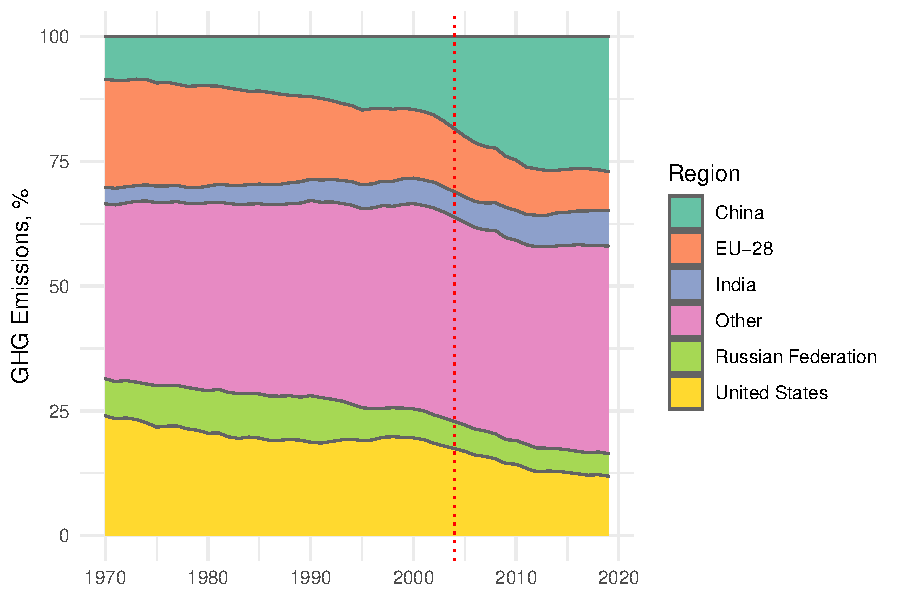
\includegraphics{Paper_files/figure-latex/unnamed-chunk-1-1.pdf}
\caption{Label TEst}
\end{figure}

\hypertarget{equity-metrics}{%
\subsubsection{Equity Metrics}\label{equity-metrics}}

\hypertarget{discussion-1}{%
\subsubsection{Discussion}\label{discussion-1}}

\hypertarget{discussion-and-conclusion}{%
\section{Discussion and Conclusion}\label{discussion-and-conclusion}}

\appendix
\section*{Appendix}
\addcontentsline{toc}{section}{Appendix}
\renewcommand{\thesubsection}{\Alph{subsection}}
\newcommand{\subsectionbreak}{\clearpage\phantomsection}
\numberwithin{table}{subsection}

\normalsize

\hypertarget{session-info-rstudio}{%
\subsection{Session Info (RStudio)}\label{session-info-rstudio}}

\footnotesize

\begin{itemize}\raggedright
  \item R version 4.2.1 (2022-06-23 ucrt), \verb|x86_64-w64-mingw32|
  \item Running under: \verb|Windows 10 x64 (build 22621)|
  \item Matrix products: default
  \item Base packages: base, datasets, graphics, grDevices, methods,
    stats, utils
  \item Other packages: dplyr~1.0.10, eurostat~3.7.10, forcats~0.5.2,
    ggplot2~3.3.6, ggridges~0.5.4, imputeTS~3.3, kableExtra~1.3.4,
    magrittr~2.0.3, openxlsx~4.2.5, pacman~0.5.1, plotly~4.10.1,
    purrr~0.3.4, readr~2.1.2, readxl~1.4.1, stringr~1.4.1,
    tibble~3.1.8, tidyr~1.2.1, tidyverse~1.3.2, WDI~2.7.8
  \item Loaded via a namespace (and not attached): assertthat~0.2.1,
    backports~1.4.1, bibtex~0.5.0, broom~1.0.1, cellranger~1.1.0,
    class~7.3-20, classInt~0.4-8, cli~3.4.0, colorspace~2.0-3,
    compiler~4.2.1, countrycode~1.4.0, crayon~1.5.1, curl~4.3.2,
    data.table~1.14.2, DBI~1.1.3, dbplyr~2.2.1, digest~0.6.29,
    e1071~1.7-11, ellipsis~0.3.2, evaluate~0.16, fansi~1.0.3,
    farver~2.1.1, fastmap~1.1.0, forecast~8.18, fracdiff~1.5-2,
    fs~1.5.2, gargle~1.2.1, generics~0.1.3, ggtext~0.1.2, glue~1.6.2,
    googledrive~2.0.0, googlesheets4~1.0.1, grid~4.2.1, gridtext~0.1.5,
    gtable~0.3.1, haven~2.5.1, here~1.0.1, highr~0.9, hms~1.1.2,
    htmltools~0.5.3, htmlwidgets~1.5.4, httr~1.4.4, jsonlite~1.8.0,
    KernSmooth~2.23-20, knitr~1.40, labeling~0.4.2, lattice~0.20-45,
    lazyeval~0.2.2, lifecycle~1.0.2, lmtest~0.9-40, lubridate~1.8.0,
    modelr~0.1.9, munsell~0.5.0, nlme~3.1-157, nnet~7.3-17,
    parallel~4.2.1, pillar~1.8.1, pkgconfig~2.0.3, plyr~1.8.7,
    proxy~0.4-27, quadprog~1.5-8, quantmod~0.4.20, R6~2.5.1,
    Rcpp~1.0.9, RefManageR~1.4.0, regions~0.1.8, reprex~2.0.2,
    rlang~1.0.5, rmarkdown~2.16, rprojroot~2.0.3, rstudioapi~0.14,
    rvest~1.0.3, scales~1.2.1, stinepack~1.4, stringi~1.7.8,
    svglite~2.1.0, systemfonts~1.0.4, tidyselect~1.1.2,
    timeDate~4021.104, tools~4.2.1, tseries~0.10-52, TTR~0.24.3,
    tzdb~0.3.0, urca~1.3-3, utf8~1.2.2, vctrs~0.4.1, viridisLite~0.4.1,
    webshot~0.5.3, withr~2.5.0, xfun~0.33, xml2~1.3.3, xts~0.12.2,
    yaml~2.3.5, zip~2.2.1, zoo~1.8-11
\end{itemize}

\normalsize
\singlespacing
\listoffigures
\listoftables

\def\bibpreamble{All online resources were last accessed on 12 December 2022.}
\footnotesize

  \bibliography{anna.bib,fabian.bib,packages.bib}

\end{document}
